\chapter{Implementation and Evaluation}
\label{Implementation_and_Evaluation}
In this chapter, we evaluate the methods presented in Chapter 3. First, the environment and the reason of using them will be explained. Then, we will show different experiments and their corresponding results.

\section{General setup}
Table~~\ref{table:Experiment_table} is a summary of all the tools and their versions in the evaluation. We use Mininet to simulate the data center network \cite{Mininet}. It allows us to creates a large-scale virtual network easily. It provides Python APIs as well as a command line interface to customize the network. It also offers an interactive interface to test the connectivity and performance.

\begin{table}[H]
\centering
\caption{Experimental environment summary}
\begin{tabular}{|l|p{4cm}|p{4.5cm}}
\hline Item & Detail version \\
\hline
\hline Operating system & Ubuntu 14.04 x86\_64 \\
\hline Controller & Ryu\_manager 4.0 \\
\hline Network Emulator & Mininet 2.2.1 \\
\hline Topology generator & Fast Network Simulation Setup (FNSS) 0.6.1\\
\hline Packet Generator & Ryu packet library API \\
\hline Southbound API & OpenFlow 1.3 \\
\hline Virtual switch & OpenvSwitch 2.5.0 \\
\hline 
\end{tabular}
\label{table:Experiment_table}
\end{table}

To evaluate the effectiveness of the detection method under various scenarios, there will be XXXX network topologies in the evaluation. They are generated by Fast Network Simulation Setup (FNSS), a Python module able to generate various types of network topology. It not only supports DCN topologies, but also provides the Mininet API, making it extremely easy to import the generated topology into Mininet. The network topologies we use are two-tier topology, three-tier topology and fat-tree topology of various sizes. The details including number of switches and average degree (i.e. the number of links between two switches) are shown in Table~~\ref{table:network_env}. The numbers in the topology name are parameters such as number of core switches, aggregation switches or edge switches, which characterize the network size. These parameters have the same meaning as the ones in \cite{FNSS}.

\begin{table}[H]
\centering
\caption{Details of network topologies}
\begin{tabular}{|l|l|l|l|}
\hline topology type & number of switches & average degree \\
\hline
\hline fat\_tree\_2 & 5 & 2 \\
\hline fat\_tree\_4 & 20 & 4 \\
\hline fat\_tree\_6 & 45 & 6 \\
\hline fat\_tree\_8 & 80 & 8 \\
\hline fat\_tree\_10 & 125 & 10 \\
\hline fat\_tree\_12 & 180 & 12 \\
\hline fat\_tree\_14 & 245 & 14 \\
\hline two\_tier\_6\_14 & 20 & 9.1 \\
\hline two\_tier\_10\_10 & 20 & 10.5 \\
\hline two\_tier\_14\_6 & 20 & 8.7 \\
\hline three\_tier\_2\_3\_5 & 20 & 2.85 \\
\hline three\_tier\_4\_2\_7 & 20 & 2.90 \\
\hline three\_tier\_4\_4\_3 & 20 & 3.40 \\
\hline three\_tier\_5\_5\_2 & 20 & 4.00 \\
\hline 
\end{tabular}
\label{table:network_env}
\end{table}

The in-band control is used for control channel. It is the default setting of Mininet and is more convenient to set up. Although there are special flow entries for in-band control channel, they are hidden and will not have any influence on our experiment. Only one controller is used. The hosts are irrelevant to our method, only a minimal number of them are in our network environment to make the topology reasonable. In fat tree topology, the number of hosts is the number of pods divided by 2, while in two-tier and three-tier topology, one host is connected to each edge switches. There are 254 flow tables in an OpenFlow switch simulated by Mininet. The flow entries are installed pro-actively in the OpenFlow switches, and due to the reason stated in the last paragraph of Section~\ref{Further_discussion}, the controller will maintain a record of switches, including ports, links and flow entries. 

The core algorithm of the flow entry detection method is implemented as a Ryu controller application. It obtains essential information from the configuration files, find aggregated groups, generate raw packets and send them by \texttt{Packet\_out}, and check \texttt{Packet\_in} to see if the packets come back as expected. Packets are generated by Ryu's built-in API library. In order to send \texttt{Packet\_out} with a raw packet, the action should be set to ``forwarding to \texttt{OFPP\_TABLE}'', which means the packet is sent to the first flow table after the action is executed; otherwise, \texttt{Packet\_out} will not be processed as an ordinary packet, and the action set will be executed directly without going through the processing pipeline \cite{PACKETOUT}. Due to the reason stated in the last paragraph of Section~\ref{Further_discussion}, the detection packets from the controller should be sent to a normal port rather than the default controller-specifying port \texttt{OFPP\_CONTROLLER}. 

\section{Flow entry generation}
\label{flow_entry_generation}
We choose common protocol fields and properly set dependency fields such as ether type, IP protocol type. The chosen fields in the field set are those that will be in our experimental network environment. The chosen set is listed as follows:

\begin{itemize}
\item
ethernet layer: eth\_dst, eth\_src
\item
ip layer: ipv4\_src, ipv4\_dst
\item
tcp/udp/icmp layer: tcp\_src, tcp\_dst, udp\_src, udp\_dst, icmpv4\_type, icmpv4\_code
\end{itemize}

The flow entries are randomly generated, and the Ryu application installs them on the switches. When a flow entry is generated, the script selects a random match field from the set of chosen match fields along with random values in a valid range and format, and selects the output port and the switch on which this entry is randomly. Due to the reason stated in Section~\ref{Further_discussion}, there will be only ``output port\_no'' action in all the flow entries. To make the scenario more realistic, the following setup is considered for flow entry generation:

\begin{itemize}
\item 
The cookie field is used as an identifier for every entry in our implementation. It is a unique integer from 0 to total entry number minus one.\sout{\red{Why mentioning cookie?}}
\item
Since the two entries with same priority that is possible to match the same packet will cause undefined behavior \cite{OF_SPEC}, the priority of entries on the same switch are different \red{Is it sufficient to set the entries with the same entries to different priorities?}.
\item
There will be duplicate field and value set deliberately generated with a 20\% chance. It is quite reasonable to have duplicates on different switches. 
\item
The IP is restricted to a /24 subnet.
\item
The number of flow entries on each switch highly depends on the forwarding policy \cite{MPFHMRSV09}. For simplicity, the number of entries on every switch is the same. 
\item
According to a firewall log found on the Internet \cite{PORT_FREQ}, the occurrence frequency of TCP ports are distributed in the following percentages to make it close to real case:
\begin{itemize}
\item
port 80: 50\%
\item
port 443: 25\%
\item
other common ports (7,20,21,22,23,25,43,53,109,110,156,161,194,546,547): 15\%
\item
other ports in 1024: 10\%
\end{itemize}
\end{itemize}

\section{Experiment and result}
In this section, we will compare the effectiveness of our method under different types of network environments. Each subsection contains different experiment designed for different purposes. The control variables including topology type, network scale, and number of flow entries will be experimented and discussed. Since our experiment involves some randomness while entries generating, the result are not always stable, especially in the small topologies. The shown result are the one that is closest to the average in 5 runs.

In statistic tables in following subsections, the effective aggregation rate is the number that the total number of entries in the network divided by total number of groups, and the actual aggregation rate is the total number of entries inside aggregated groups divided by total number of groups, both of them are affected by only the regular entries in the environment, which do not include the auxiliary entries. Due to the fact that entries that has other entries with same match field and value may belong to more than one aggregated group, the total entries in groups will be more than the total entries exist in the network. The aggregation rates number will be rounded to the second decimal place.

When an auxiliary entry is installed, a short period of waiting time is needed, otherwise after the Packet\_Out is send, there is a low chance that it might be forwarded unexpectedly. This happens when it arrives at an certain switch that contains an auxiliary entry, the entry is not installed. Therefore, for every installation of auxiliary entry, the controller will wait 0.01 second before continuing the process to ensure the auxiliary entries work as expected. The time for adding auxiliary flow entries is included in execution time. In the statistics, time will also be rounded to the second decimal place. The number of auxiliary entries is also calculated.

\subsection{Influence of topology type}
In order to see the influence of topology type, we select 8 different topologies with the same number of 20 switches from Table~~\ref{table:network_env} with 20 entries on each switch. The topologies including one fat tree topology, three two-tier topologies and four three-tier topologies are listed along with their experimental result in Table~~\ref{table:different_topo_type}. The bar chart of effective aggregation rate of these topologies are in Figure~\ref{different_topo_bar}.

\begin{table}
\centering
\caption{Influence of different topology types}
\begin{tabular}{|l|p{2.5cm}|p{2.5cm}|p{1.9cm}|p{2.8cm}|}
\hline topology name & Effective aggregation rate & Actual aggregation rate & Execution time(sec) & Number of auxiliary entry \\
\hline fat\_tree\_4 & 2.96 & 3.27 & 8.27 & 142 \\
\hline two\_tier\_6\_14 & 1.77 & 1.82 & 6.69 & 262 \\ 
\hline two\_tier\_10\_10 & 2.70 & 3.04 & 7.96 & 182 \\
\hline two\_tier\_14\_6 & 2.72 & 3.81 & 9.57 & 109 \\ 
\hline three\_tier\_2\_3\_5 & 1.44 & 1.49 & 6.23 & 290 \\
\hline three\_tier\_4\_2\_7 & 1.35 & 1.56 & 6.61 & 271 \\
\hline three\_tier\_4\_4\_3 & 1.83 & 2.03 & 7.72 & 232 \\
\hline three\_tier\_5\_5\_2 & 2.21 & 2.51 & 7.63 & 184 \\
\hline
\end{tabular}
\label{table:different_topo_type}
\end{table}

\begin{figure}[H]
\begin{center} 
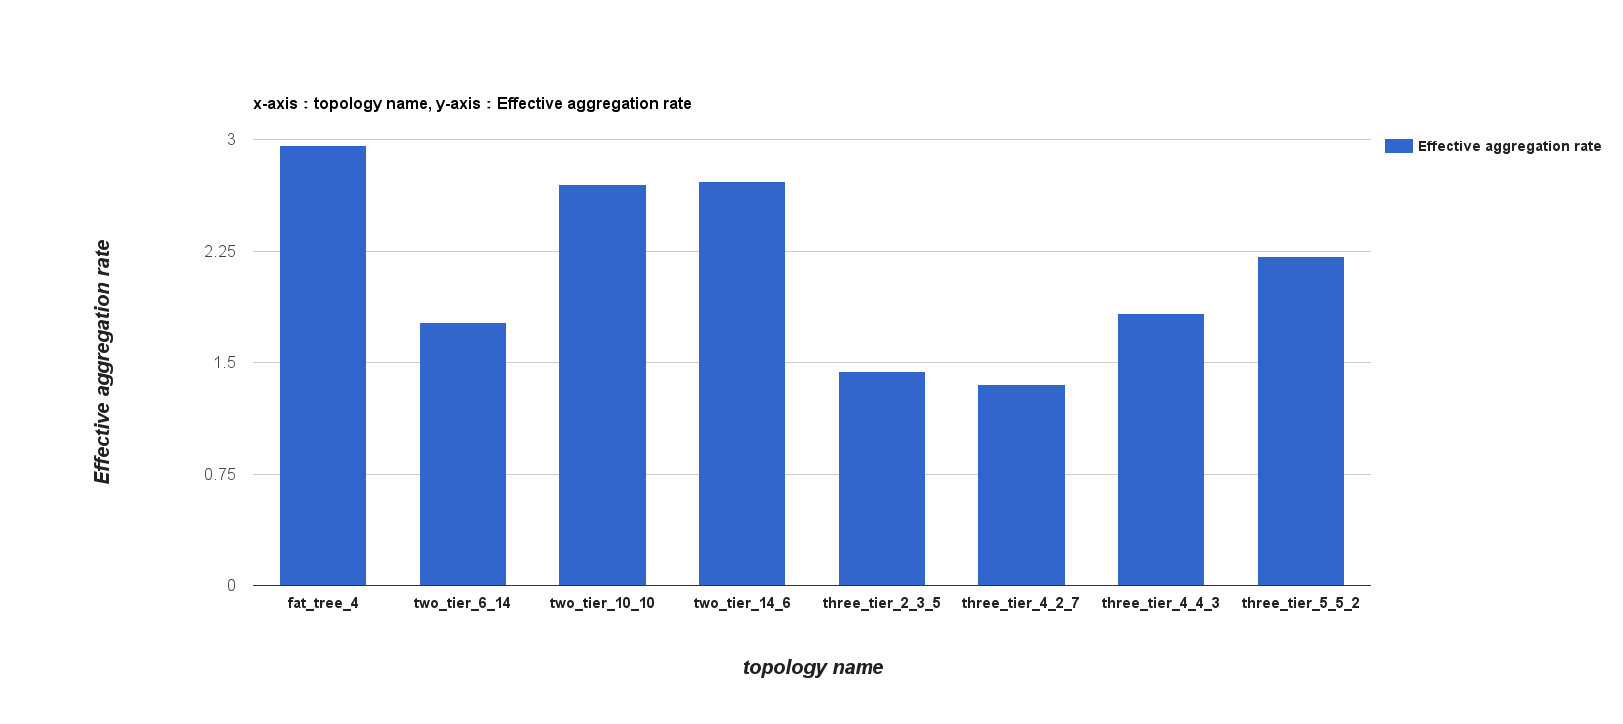
\includegraphics[width=1.4\linewidth]{figures/exp_topotype_bar.png}
\end{center}
\caption{The bar chart of different topologies.}
\label{different_topo_bar}
\end{figure}

In order to further analyze the result, we select the most effective one, fat\_tree\_4, and the least effective one, three\_tier\_4\_2\_7, and find the distribution of the number of groups that contain certain number of entries, which is shown as Figure~\ref{different_topo_distribute}. The x-axis is the number of entries an aggregated group contains, and the y-axis is the number of groups that contain certain number of entries.

\begin{figure}[H]
\begin{center} 
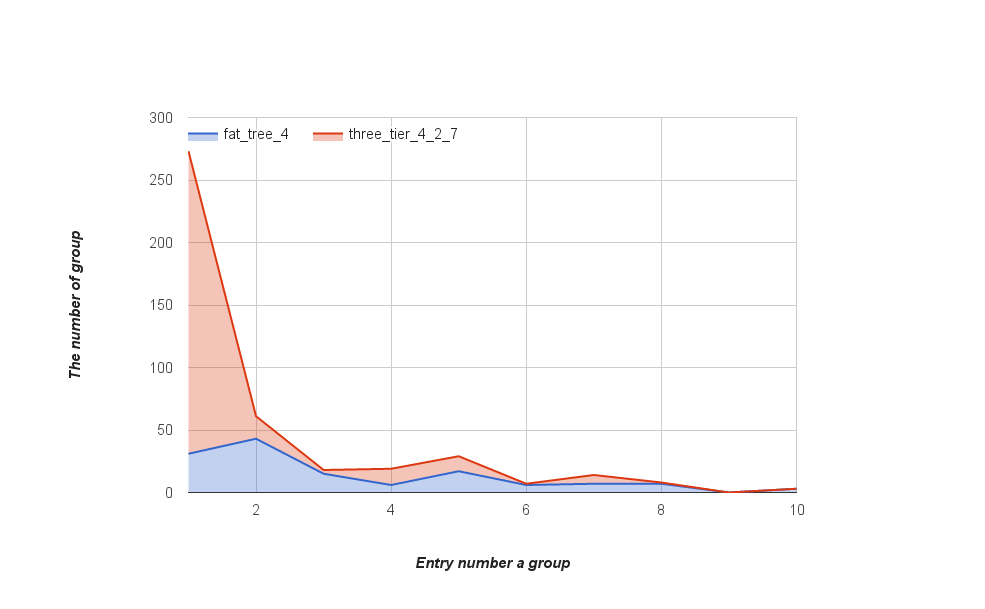
\includegraphics[width=1.4\linewidth]{figures/exp_topotype_distribute.png}
\end{center}
\caption{The comparison between fat\_tree\_4 and three\_tier\_4\_2\_7 - the number of aggregated groups than contains different number of entries.}
\label{different_topo_distribute}
\end{figure}

\subsection{Influence of network scale}
To observe how effective our method is under different network scales, different sizes of fat tree topology will be used. Fat tree topologies are chosen for this experiment because the other two types of topology has influence the result of the experiment mostly by the way switches are connected, please refer to the rest of the conclusion in the third paragraph of \ref{examination_and_discussion}. The parameter $n$, denoting the number of pods, will be from 2 to 14. Since the network scale grows significantly with higher pod number, we will only at most 14 pod at max. There are also 20 entries on each switch. The results are shown in Table~~\ref{table:different_scale}, and the trend chart of effective aggregation rate and actual aggregation rate are shown in Figure~\ref{different_scale_rate_trend}.

\begin{table}
\centering
\caption{Influence of different network scales}
\begin{tabular}{|l||l|l|l|l|}
\hline topology name & Effective aggregation rate & Actual aggregation rate & Execution time(sec) & Number of auxiliary entry \\
\hline
\hline fat\_tree\_2 & 2.70 & 2.84 & 1.26 & 35 \\
\hline fat\_tree\_4 & 2.96 & 3.27 & 8.27 & 142 \\
\hline fat\_tree\_6 & 2.85 & 3.27 & 19.16 & 327 \\
\hline fat\_tree\_8 & 2.81 & 3.29 & 33.03 & 589 \\
\hline fat\_tree\_10 & 2.91 & 3.37 & 51.81 & 921 \\
\hline fat\_tree\_12 & 2.89 & 3.36 & 74.78 & 1334 \\
\hline fat\_tree\_14 & 2.79 & 3.29 & 102.56 & 1800 \\
\hline
\end{tabular}
\label{table:different_scale}
\end{table}

\begin{figure}[H]
\begin{center} 
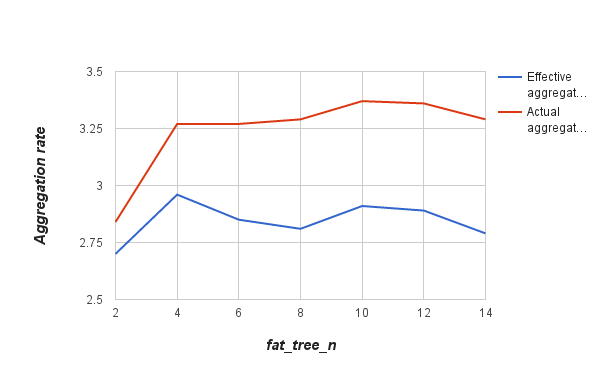
\includegraphics[width=1\textwidth]{figures/exp_scale_rate_trend.png}
\end{center}
\caption{The trend chart of aggregation rates under different scale of network.}
\label{different_scale_rate_trend}
\end{figure}

The relation between topology size and execution time is in Figure~\ref{different_scale_time_trend}, and the relation between topology size and the number of auxiliary entries is in Figure~\ref{different_scale_aux_trend}. As we can see, both trend looks pretty similar, they are proportional to the square of $n$. It is quite as expected since the growth rate of switch is also proportional to the square of $n$.

\begin{figure}[H]
\begin{center} 
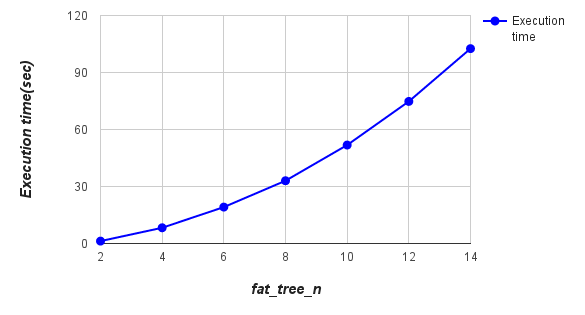
\includegraphics[width=1\textwidth]{figures/exp_scale_time_trend.png}
\end{center}
\caption{The trend chart of execution time under different scale of network.}
\label{different_scale_time_trend}
\end{figure}

\begin{figure}[H]
\begin{center} 
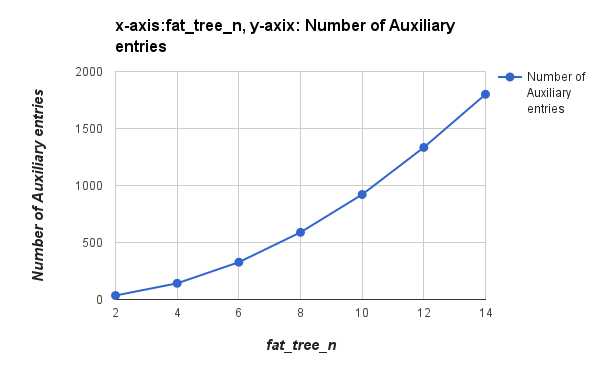
\includegraphics[width=1\textwidth]{figures/exp_scale_aux_trend.png}
\end{center}
\caption{The trend chart of number of auxiliary entries under different scale of network.}
\label{different_scale_aux_trend}
\end{figure}

\subsection{Influence of flow entry number}
In this experiment, we will use only one topology - fat\_tree\_4 and change the number of entries on each switch to see the influence it might bring. The number of entries on each switch increases 5 entries from 5 to 50 every run, and the increasing number grows in the interval from 50 to 200. The result table is in Table~~\ref{table:different_entry_per_switch}, and the trend chart of effective aggregation rate with different number of entries on each switch is shown as Figure~\ref{exp_entrynum_trend}. The execution time and the number of auxiliary grow linearly along with the number of entries on a switch.

\begin{table}
\centering
\caption{Different number of entries in a switch.}
\begin{tabular}{|l|p{2.6cm}|p{2.6cm}|p{1.9cm}|p{2.8cm}|}
\hline Number of entries per switch & Effective aggregation rate & Actual aggregation rate & Execution time (sec) & Number of auxiliary entry \\
\hline
\hline 5 & 2.27 & 2.66 & 1.64 & 36 \\
\hline 10 & 2.38 & 2.82 & 3.98 & 72 \\
\hline 15 & 2.59 & 2.91 & 5.53 & 110 \\
\hline 20 & 2.96 & 3.27 & 8.27 & 142 \\
\hline 25 & 2.94 & 3.29 & 11.08 & 179 \\
\hline 30 & 3.14 & 3.55 & 15.03 & 214 \\
\hline 35 & 3.19 & 3.58 & 17.22 & 242 \\
\hline 40 & 3.36 & 3.72 & 19.24 & 280 \\
\hline 45 & 3.37 & 3.80 & 24.42 & 310 \\
\hline 50 & 3.45 & 3.86 & 26.19 & 346 \\
\hline 65 & 3.35 & 3.75 & 34.31 & 461 \\
\hline 80 & 3.40 & 3.77 & 41.47 & 560 \\
\hline 100 & 3.50 & 3.92 & 55.58 & 672 \\
\hline 120 & 3.53 & 3.98 & 64.96 & 812 \\
\hline 140 & 3.55 & 3.96 & 79.21 & 977 \\
\hline 160 & 3.58 & 4.01 & 89.21 & 1070 \\
\hline 180 & 3.53 & 3.94 & 102.54 & 1216 \\
\hline 200 & 3.60 & 4.02 & 119.47 & 1359 \\
\hline 
\end{tabular}
\label{table:different_entry_per_switch}
\end{table}

\begin{figure}[H]
\begin{center} 
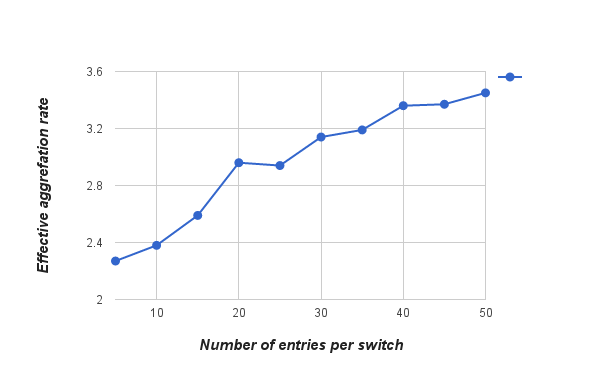
\includegraphics[width=1\textwidth]{figures/exp_entrynum_trend.png}
\end{center}
\caption{The trend chart of effective aggregation rate with different number of entries on every switch.}
\label{exp_entrynum_trend}
\end{figure}

\subsection{Examination and discussion}
\label{examination_and_discussion}
From the result in Table~~\ref{table:different_topo_type} and Figure~\ref{different_topo_bar}, we can tell that although the number of switches are the same, the way how they are connected to each other leads to significant differences. Generally, we expect that the higher degree is, the higher is the chance that we are able to extend an aggregation group more, which should result in higher aggregation rates. However, it seems that it is not always true, since according to our result, the two-tier topologies has the highest average degree overall but has moderate result, the fat tree topology has the best result, while the three-tier topologies tend to have worse result. 

After tracking down the entry inside the two-tier topologies, we discover that although the degree number is high, the ratio between the number of forwarding ports and the number of entries is imbalanced. Since the ports forwarding to different neighbor is distributed equally among entries, and in fact, they are the real routing options for an aggregated group to choose, there are not as many options as we may think, and causes the fact that the aggregation rates of two tier topologies are lower than that of the fat tree topology. 

In the Figure~\ref{different_topo_distribute}, we can see two things: first, the area coverage of the trend chart of three\_tier\_4\_2\_7 is apparently larger than fat\_tree\_4. Since in this experiment, there are same number of switches and entries in every topologies, this can mean that the groups contain more redundant entries caused by the entries with same match field an value. However, it should not be the reason for bad aggregation rates in three-tier topologies since this affects the execution time more than aggregation rate, and in Table~~\ref{table:different_topo_type}, the difference of effective aggregation rate and actual aggregation rate of the fat tree topology is even slightly larger than that of the three-tier topology. Second, a lot of groups in three\_tier\_2\_7 only contain one entry. This is induced by the fact that the aggregation switches being the hub node in the topology. In the middle of the aggregated group finding stage, after a few aggregation groups with many entries are formed, and the entries in the aggregation switches belong to certain group, the rest of the entries in the core switches and edge switched are cut off and not able to connect in order to form another big group. And it is even more so in three\_tier\_4\_2\_7 since compare to other three-tier topologies, there are only two aggregation switches.
This can explain the bad aggregation rate in these topologies.

In the trend chart of effective aggregation rate and actual aggregation rate in Figure~\ref{different_scale_rate_trend}, except fat\_tree\_2 who has lower aggregation rates due the less number of switches and links 
the aggregation rates are similar in different sizes of topology, it actually does not have any clear effect on the aggregation rate. Theoretically, there should be positive factors and negative factors that would influence the aggregation rates. A positive factor, for example, is the larger number of links, which helps to raise the chance for adopting an entry into a grow if the ratio between the number of forwarding ports and entries are balanced. And examples of negative factors including more entries to be fit into aggregated groups, and more hosts that will stop an aggregated group from extending. The result show that these factors break even, and the effectiveness of our method will not drop with the increasing of size of topologies.

From the trend chart Figure~\ref{exp_entrynum_trend}, we can clearly see that the aggregation rate grows as the number of entries in the switch increases from 5 to 50 entries per switch. However, the growth rate slowly decreases after 40 entry per switch and converges as the number of entry gets larger and larger. 
A reasonable explanation for this phenomenon is the limitation of the number of fields a detection packet has. According to the selected field set in \ref{flow_entry_generation}, XXXXXXXXXXX
And as a detection packet get more close to saturation, it will also make it harder for the corresponding aggregated group to find another entry that satisfies the aggregation conditions. 

In order to justify the inference, we also did another run of experiment with 500 entries on each switch, which results in 3.99 effective aggregation rate and 4.3 actual aggregation rate.

With these analysis, we can conclude that the more entries are in the switches, the higher aggregation rates we are able to get, but this is only true before the fields of detection packet reaches saturation. 